\section{Evaluation}

The results of the PAN~2010 competition~\cite{Potthast2010b}
provides a benchmark of comparison for vandalism detection systems.
Although receiver operating characteristic was used to judge the
competition, the analysis by Potthast~\etal points to the conclusion
that the class imbalance between vandalized and regular edits
leads to better discriminatory power by precision-recall curves.

\begin{figure}[tbhp]
  \centering
  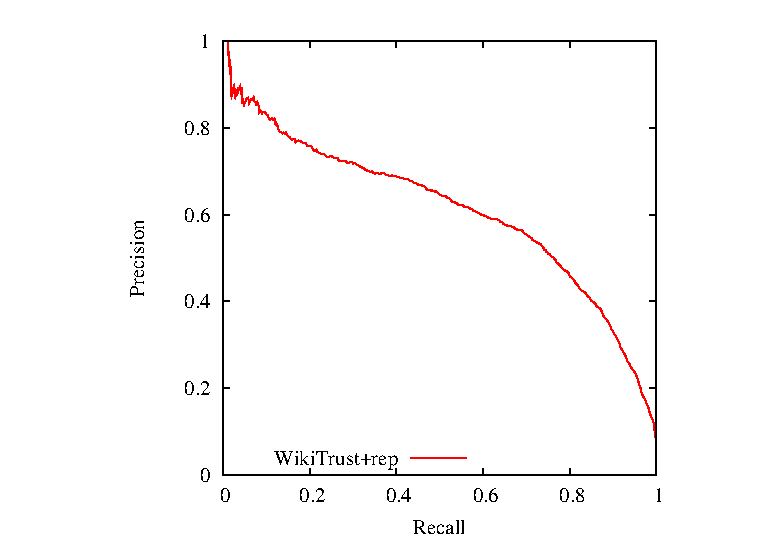
\includegraphics{part-Q10-vandalism/graph-wikitrust-pr}
  \caption[Precision-Recall curve for vandalism detection]{%
    Precision-Recall curve for a vandalism detection system based
    on features from the WikiTrust system, including reputation.
    This extends the previous WikiTrust results for immediate vandalism
    detection~\cite{Adler2010b} by including the reputation of authors
    at the time of each edit.}
\end{figure}

\begin{table}[tbhp]
    \begin{center}
        \begin{tabular}{|l|c|c|}
\hline
\textbf{System} & \textbf{AUC-PR} & \textbf{AUC-ROC} \\
\hline
\hline
PAN~2010 WikiTrust~\cite{Potthast2010b} & 0.49263 & 0.90351 \\
STiki (Metadata)~\cite{Adler2011a} & 0.52534 & 0.91520 \\
PAN 2010 WikiTrust + length~\cite{Adler2011a} & 0.61047 & 0.93647 \\
PAN 2010 WikiTrust + reputation & 0.61152 & 0.94257 \\
Mola-Velasco (NLP)~\cite{Adler2011a} & 0.73121 & 0.94567 \\
Mola-Velasco + topic~\cite{Mola2011} & 0.7541 & \textit{n/a} \\
PAN'10 Meta Detector~\cite{Potthast2010b} & 0.77609 & 0.95689 \\
M-V + WT + STiki~\cite{Adler2011a} & 0.81829 & 0.96902 \\
\hline
        \end{tabular}
    \end{center}
    \caption{Comparison of various vandalism detection systems.}
\end{table}
